\documentclass{standalone}
\usepackage{tikz}
\usepackage{amsmath}
\usepackage{amssymb}
\usepackage{tgtermes}
\usepackage{newtxtext}
\usepackage{newtxmath}
\usetikzlibrary{arrows.meta, positioning, calc, backgrounds}

\begin{document}
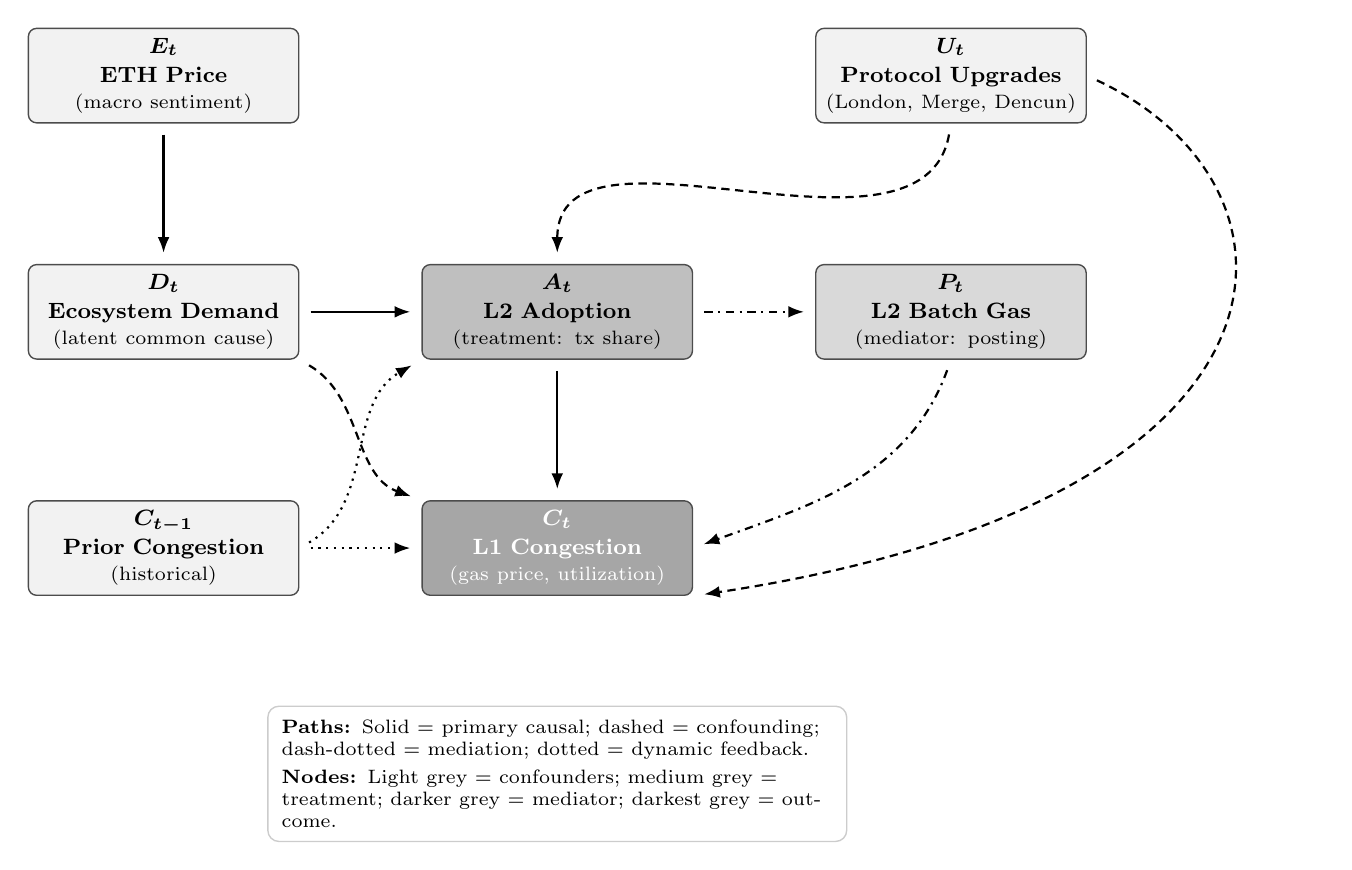
\begin{tikzpicture}[
  node distance = 3cm and 5cm,
  every node/.style = {
    rounded corners=3pt,
    draw=black!70,
    align=center,
    font=\footnotesize,
    fill=white,
    minimum height=1.2cm,
    text width=3.2cm,
    line width=0.5pt
  },
  arrow/.style = {-{Latex[length=2mm]}, line width=0.8pt, shorten >=4pt, shorten <=4pt},
  confounder/.style = {fill=gray!10},
  mediator/.style = {fill=gray!30},
  treatment/.style = {fill=gray!50},
  outcome/.style = {fill=gray!70, text=white}
]

% Layer 1: Macro drivers (top row)
\node[confounder] (E) at (0,0) {$\boldsymbol{E_t}$\\[1pt]\textbf{ETH Price}\\{\scriptsize (macro sentiment)}};

\node[confounder] (U) at (10,0) {$\boldsymbol{U_t}$\\[1pt]\textbf{Protocol Upgrades}\\{\scriptsize (London, Merge, Dencun)}};

% Layer 2: Ecosystem demand (left side)
\node[confounder] (D) at (0,-3) {$\boldsymbol{D_t}$\\[1pt]\textbf{Ecosystem Demand}\\{\scriptsize (latent common cause)}};

% Layer 3: Treatment (center)
\node[treatment] (A) at (5,-3) {$\boldsymbol{A_t}$\\[1pt]\textbf{L2 Adoption}\\{\scriptsize (treatment: tx share)}};

% Layer 4: Mediator (right side)
\node[mediator] (P) at (10,-3) {$\boldsymbol{P_t}$\\[1pt]\textbf{L2 Batch Gas}\\{\scriptsize (mediator: posting)}};

% Layer 5: Dynamic feedback (bottom left)
\node[confounder] (Cprev) at (0,-6) {$\boldsymbol{C_{t-1}}$\\[1pt]\textbf{Prior Congestion}\\{\scriptsize (historical)}};

% Layer 6: Outcome (bottom center)
\node[outcome] (C) at (5,-6) {$\boldsymbol{C_t}$\\[1pt]\textbf{L1 Congestion}\\{\scriptsize (gas price, utilization)}};

% === ARROWS (without overlapping labels) ===

% Primary causal paths (solid)
\draw[arrow] (E.south) -- (D.north);
\draw[arrow] (D.east) -- (A.west);
\draw[arrow] (A.south) -- (C.north);

% Confounding paths (dashed)
\draw[arrow, densely dashed] (D.south east) to[out=-30, in=160] (C.north west);
\draw[arrow, densely dashed] (U.south) to[out=-100, in=90] (A.north);
\draw[arrow, densely dashed]
  (U.east)
  .. controls ($(P.east)+(3.0cm,1.6cm)$) and ($(P.east)+(3.0cm,-2.4cm)$)
  .. (C.south east);

% Mediation paths (dash-dotted)
\draw[arrow, dashdotted] (A.east) -- (P.west);
\draw[arrow, dashdotted] (P.south) to[out=-110, in=20] (C.east);

% Dynamic feedback (dotted)
\draw[arrow, dotted] (Cprev.east) to[out=30, in=-150] (A.south west);
\draw[arrow, dotted] (Cprev) -- (C);

% === LEGEND ===
\node[draw=gray!40, fill=white, rounded corners=4pt,
      font=\scriptsize, align=left, text width=7cm,
      anchor=north, inner sep=5pt, line width=0.5pt]
      at (5,-8) {
    \textbf{Paths:} Solid = primary causal;
    dashed = confounding;
    dash-dotted = mediation;
    dotted = dynamic feedback.\\[2pt]
    \textbf{Nodes:} Light grey = confounders;
    medium grey = treatment;
    darker grey = mediator;
    darkest grey = outcome.
};

\end{tikzpicture}
\end{document}
